\documentclass{scrartcl}

\usepackage{makeidx}
\usepackage[cache]{minted}
\usepackage{tikz}
\usepackage{colortbl}
\usepackage{mfirstuc}
\usepackage{tabu}
\usepackage{fancyvrb}
\usepackage{hyperref}

\hypersetup{
    colorlinks=true,
    linkcolor=blue!80,
    filecolor=magenta,
    urlcolor=blue!80,
}

% \usepackage{etoolbox}
% \let\originalinput\input
% \newcommand{\newinput}[1]{\InputIfFileExists{#1}{}{}}
% \AtBeginEnvironment{tabu*}{\let\input\newinput}

\usetikzlibrary{positioning, calc, sbgn}

\tikzset{sbgn/.append style={execute at begin picture={
    \pgfdeclarelayer{includedcompartments}
    \pgfsetlayers{background,compartments,includedcompartments,nodes,arcs,subcomplexes,subunits,attributes,main}}
    }
}

\def\texttikz{Ti\textit{k}Z}
\def\textpgf{\texttt{PGF}}
\def\tikzmanual{\textpgf/\texttikz{} manual}
\def\sbgntikz{SBGN\texttikz}

\def\colkey#1{\textcolor{red!80}{\texttt{#1}}}

\newenvironment{entry}[3]
{
    \noindent\glyph{#1}{#2}{#3}
    \begin{flushright}
    \begin{minipage}[c]{0.95\linewidth}
}
{
    \end{minipage}
    \end{flushright}
    % \vspace{0.5cm}
}

\def\glyph#1#2#3{
    \index{\MakeLowercase #1}
    \large\textsf{#1 (#3)}\normalsize \hfill \colkey{/tikz/#2}
}

% Shamelessly stolen from minted manual's source code ;)
\newenvironment{code}
{
    \vskip5pt
    \VerbatimEnvironment
    \begin{VerbatimOut}{code.out}%
}
{
    \end{VerbatimOut}%
    \colorbox{blue!10}{
        \begin{minipage}[c]{0.33\textwidth}
        \center
        \scalebox{0.8}{
        \begin{tikzpicture}[sbgn]
            \input{code.out}
        \end{tikzpicture}
        }
    \end{minipage}}
    \colorbox{gray!10}{
        \begin{minipage}[c]{0.60\textwidth}%
        \inputminted[resetmargins, breaklines, fontsize = \footnotesize]{latex}{code.out}%
    \end{minipage}}
    \vskip5pt
}

\title{sbgntikz}
\subtitle{manual for version 1.1.*}
\author{Adrien Rougny}

\makeindex

\begin{document}

\maketitle

\begin{center}
\scalebox{0.35}{
    \begin{tikzpicture}[sbgn,
        simple chemical/.append style={fill=blue!40},
        complex/.append style={fill=red!40},
        macromolecule/.append style={fill=orange!40},
        phenotype/.append style={fill=green!40},
        submap/.append style={fill=yellow!40},
        compartment/.append style={fill=brown!10}]

    \node[macromolecule] (subigf) {IGF};
    \node[macromolecule, below = 0.1cm of subigf] (subigfr) {IGFR};
    \node[complex, subunits = (subigf)(subigfr)] (comp) {};
    \node[macromolecule] (subigf) {IGF};
    \node[macromolecule, below = 0.1cm of subigf] (subigfr) {IGFR};

    \node[association, connectors = horizontal, left = of comp.200] (p1) {};

    \node[macromolecule, left = of p1] (igfr) {IGFR};

    \node[macromolecule, above left = 3cm and 1.5cm of p1] (igf) {IGF};

    \node[generic process, connectors = horizontal, below = 3.5cm of comp] (p2) {};

    \node[macromolecule, left = of p2] (irs1-4) {IRS1-4};
    \node[sv] at (irs1-4.north) {};

    \node[macromolecule, right = of p2] (pirs1-4) {IRS1-4};
    \node[sv] at (pirs1-4.north) {P};

    \node[simple chemical, clone, above left = of p2] (atp1) {ATP};

    \node[simple chemical, clone, above right = of p2] (adp1) {ADP};

    \node[generic process, connectors = horizontal, below = of pirs1-4] (p3) {};

    \node[macromolecule, right = of p3] (inactivegrb2) {Grb2};
    \node[sv] at (inactivegrb2.south) {inactive};

    \node[macromolecule, left = of p3] (activegrb2) {Grb2};
    \node[sv] at (activegrb2.south) {active};

    \node[association, connectors = vertical, below left = of activegrb2] (p4) {};

    \node[macromolecule, above left = of p4] (sos) {SOS};

    \node[macromolecule subunit, below right = 1.7cm and 0.05cm of p4.south] (sub-activegrb2) {Grb2};
    \node[sv] at (sub-activegrb2.south) {active};
    \node[macromolecule subunit, below left = 1.7cm and 0.05cm of p4.south] (sub-sos) {SOS};
    \node[complex, subunits = (sub-sos)(sub-activegrb2)] (comp2) {};
    \node[macromolecule subunit, below right = 1.7cm and 0.05cm of p4.south] (sub-activegrb2) {Grb2};
    \node[sv] at (sub-activegrb2.south) {active};
    \node[macromolecule subunit, below left = 1.7cm and 0.05cm of p4.south] (sub-sos) {SOS};

    \node[generic process, connectors = horizontal, below = of comp2] (p5) {};

    \node[macromolecule, left = of p5] (inactiveras) {RAS};
    \node[sv] at (inactiveras.south) {inactive};

    \node[macromolecule, right = of p5] (activeras) {RAS};
    \node[sv] at (activeras.south) {active};

    \node[simple chemical, below left = of p5] (gtp) {GTP};

    \node[simple chemical, below right = of p5] (gdp) {GDP};

    \node[submap, right = 0.75cm of activeras, align = center, minimum width = 200pt, minimum height = 100pt, fill = yellow!50] (submap) {MAPK\\cascade};

    \node[tag, orientation = right, anchor = west, fill = yellow!50] at (submap.west) (tagras) {RAS};

    \node[tag, orientation = left, anchor = east, fill = yellow!50] at (submap.east) (tagerk) {ERK};

    \node[macromolecule, right = 0.75cm of submap] (2perk) {ERK};
    \node[sv] at (2perk.220) {2P};

    \node[generic process, connectors = horizontal, above right = 3.5cm and 3cm of 2perk] (p6) {};

    \node[macromolecule, left = of p6] (rsk) {RSK};
    \node[sv] at (rsk.north) {};

    \node[macromolecule, right = 4.5cm of p6] (prsk) {RSK};
    \node[sv] at (prsk.north) {P};

    \node[simple chemical, clone, above left = of p6] (atp2) {ATP};

    \node[simple chemical, clone, above right = of p6] (adp2) {ADP};

    \node[generic process, connectors = horizontal, below = 3.5cm of prsk] (p7) {};

    \node[macromolecule, left = of p7] (c-fos) {c-Fos};
    \node[sv] at (c-fos.north) {};

    \node[macromolecule, right = of p7] (pc-fos) {c-Fos};
    \node[sv] at (pc-fos.north) {P};

    \node[simple chemical, clone, above left = of p7] (atp3) {ATP};

    \node[simple chemical, clone, above right = of p7] (adp3) {ADP};

    \node[phenotype, below = of pc-fos, align = center] (pheno) {gene\\transcription};

    \draw[consumption] (igf) -- (p1.west);
    \draw[consumption] (igfr) -- (p1.west);
    \draw[production] (p1.east) -- (comp.200);
    \draw[catalysis] (comp) -- (p2);
    \draw[consumption] (atp1) -- (p2.west);
    \draw[consumption] (irs1-4) -- (p2.west);
    \draw[production] (p2.east) -- (adp1);
    \draw[production] (p2.east) -- (pirs1-4);
    \draw[stimulation] (pirs1-4) -- (p3);
    \draw[consumption] (inactivegrb2) -- (p3.east);
    \draw[production] (p3.west) -- (activegrb2);
    \draw[consumption] (activegrb2) -- (p4.north);
    \draw[consumption] (sos) -- (p4.north);
    \draw[production] (p4.south) -- (comp2);
    \draw[stimulation] (comp2) -- (p5);
    \draw[consumption] (inactiveras) -- (p5.west);
    \draw[consumption] (gtp) -- (p5.west);
    \draw[production] (p5.east) -- (activeras);
    \draw[production] (p5.east) -- (gdp);
    \draw[equivalence arc] (activeras) -- (tagras);
    \draw[equivalence arc] (tagerk) -- (2perk);
    \draw[catalysis] (2perk) -| (p6);
    \draw[consumption] (rsk) -- (p6.west);
    \draw[consumption] (atp2) -- (p6.west);
    \draw[production] (p6.east) -- (prsk);
    \draw[production] (p6.east) -- (adp2);
    \draw[catalysis] (prsk) -- (p7);
    \draw[consumption] (c-fos) -- (p7.west);
    \draw[consumption] (atp3) -- (p7.west);
    \draw[production] (p7.east) -- (pc-fos);
    \draw[production] (p7.east) -- (adp3);
    \draw[stimulation] (pc-fos) -- (pheno);
    \draw[compartment, rounded corners=10pt] let \p1=(comp.160), \p2=(igfr.west), \p3=(pheno.south east), \p4=(comp.20) in
    (\p1) -- ($(\x2,\y1)+(-1cm,0)$)
    -- ($(\x2,\y3)+(-1cm,-1cm)$)
    -- ($(\x3,\y3)+(1cm,-1cm)$)
    -- ($(\x3,\y4)+(1cm,0)$)
    -- (\p4)
    node[below, pos = 0.8] {\huge cytosol}
    ;
    \draw[compartment, rounded corners=10pt] let \p1=(comp.150), \p2=(igfr.west), \p3=(pheno.south east), \p4=(comp.30), \p5=(igf.north) in
    (\p1) -- ($(\x2,\y1)+(-1cm,0)$)
    -- ($(\x2,\y5)+(-1cm,1cm)$)
    -- ($(\x3,\y5)+(1cm,1cm)$)
    node[below, pos = 0.46] {\huge extracelullar}
    -- ($(\x3,\y4)+(1cm,0)$)
    -- (\p4)
    ;


\end{tikzpicture}
}

\scriptsize Map adapted from SBGN PD language L1V1.3, Journal of Integrative Bioinformatics, 2015 Sep 4;12(2):263 \normalsize
\end{center}

\newpage

\tableofcontents

\section{Introduction}

\subsection{About}

\emph{sbgntikz} is a \texttikz~\cite{tikz} library to draw SBGN PD, AF or ER maps~\cite{sbgn} directly into \LaTeX{} documents.
It basically encodes SBGN glyphs into \texttikz{} shapes and arrowheads named by keywords, making them straightforwardly drawable within a \texttikz{} picture.
Drawing a specific glyph is then as simple as specifying its corresponding keyword in some \texttikz{} command.

The present manual is intended for an audience that knows SBGN but not particularly \texttikz{}.
The rest of the present section is dedicated to the first steps in using \emph{sbgntikz}: installing the library and drawing a first map (while introducing some basic \texttikz{} syntax).
Section~\ref{sec:draw} references all glyphs and their associated keywords, whereas section~\ref{sec:eff} gives some \texttikz{} options and syntaxes that I find most useful to draw SBGN maps.
I believe users already familiar with \texttikz{} will mostly be interested in reading section~\ref{sec:draw}, and might have different (and maybe better) solutions to the issues presented in section~\ref{sec:eff}.

\subsection{Installation and usage}

The directory \mintinline{bash}{tikz-sbgn/} should be copied to a directory where it can be found by the \TeX{} engine:
\begin{itemize}
    \item in the directory of your \LaTeX{} source file
    \item in your local \mintinline{bash}{texmf} directory. This directory is usually \mintinline{bash}{/home/<user>/texmf/} under Linux, \mintinline{bash}{/Users/Library/texmf/} under MacOS, and \mintinline{bash}{C:/Users/<user>/texmf} under Windows, but it can depend on your OS version and \TeX{} distribution. Your \mintinline{bash}{texmf} directory can be found using the \mintinline{bash}{kpsewhich -var-value=TEXMFHOME} command.
\end{itemize}

Usually, \texttikz{} is installed within your \TeX{} distribution, so \texttikz{} and \emph{sbgntikz} can be imported directly into your \LaTeX{} source file with no further installation adding the following two commands to your preamble:

\begin{minted}[bgcolor=gray!10]{latex}
\usepackage{tikz}
\usetikzlibrary{sbgn}
\end{minted}

An SBGN map can then be drawn within a \texttikz{} picture using the \colkey{sbgn} key:

\begin{minted}[bgcolor=gray!10]{latex}
\begin{tikzpicture}[sbgn]
% tikz code to draw an SBGN map
\end{tikzpicture}
\end{minted}

\subsection{A first map}

SBGN is all about drawing nodes with specific shapes and arcs with specific arrow heads.
Fortunately, drawing \texttikz{} pictures is not different, making it pretty straightforward to draw SBGN maps using \emph{sbgntikz}: the \mintinline{tex}{\node} command is used to draw nodes, while the \mintinline{tex}{\draw} command is used to draw arcs.
The code to draw an SBGN node (or an attribute) will usually look like the following:

\begin{minted}[bgcolor=gray!10]{latex}
\node[<sbgn node>, ...] (name) at (point) {LABEL};
\end{minted}

where
\begin{itemize}
\item \mintinline{latex}{<sbgn node>} is a keyword corresponding to the type of node to be drawn (e.g. \mintinline{latex}{simple chemical} for a simple chemical);
\item \mintinline{latex}{...} is a list of other options for the node (e.g. its relative positioning towards another node, color, line width \dots);
\item \mintinline{latex}{(name)} specifies the name of the node (optional);
\item \mintinline{latex}{at (point)} specifies the point on the canvas where to draw the node (optional, by default \mintinline{latex}{(0,0)} if no relative positioning is specified in the nodes' options);
\item \mintinline{latex}{{LABEL}} specifies the label of the node that will be displayed (mandatory but can be empty).
\end{itemize}

As for arcs, they can be drawn using the following piece of code:

\begin{minted}[bgcolor=gray!10]{latex}
\draw[<sbgn arc>, ...] (a) -- (b);
\end{minted}

where

\begin{itemize}
\item \mintinline{latex}{<sbgn arc>} is a keyword corresponding to the type of arc to be drawn (e.g. \mintinline{latex}{necessary stimulation} for a necessary stimulation);
\item \mintinline{latex}{...} is a list of other options for the arc (e.g. its color, line width \dots);
\item \mintinline{latex}{(a)} is a point on the canvas or the name of a node from which the arc will depart;
\item \mintinline{latex}{(b)} is a point on the canvas or the name of a node on which the arc will arrive.
\end{itemize}

Knowing those two basic syntaxes, one can draw pretty much any desired SBGN map.
Following is an example of code to draw a simple PD map.
It relies on relative positioning provided by \texttikz{}'s \mintinline{tex}{positioning} library, as positioning all nodes with absolute coordinates would be too cumbersome (see section~\ref{sec:eff} for few more details, or the \tikzmanual{} for lot more details).


\begin{center}
\scriptsize
\begin{minted}[bgcolor=gray!10, breaklines = true]{latex}
\documentclass{standalone}

\usepackage{tikz}
\usetikzlibrary{positioning, sbgn}

\begin{document}

\begin{tikzpicture}[sbgn]
\node[macromolecule] (erk) {ERK};   % this node has no absolute nor relative positioning, so it is placed at (0,0) by default
\node[sv] at (erk.120) {};  % the state variable is placed on the border of the node, at an angle of 120 deg
\node[generic process, connectors = horizontal, right = of erk] (p) {}; % we add connectors, and use relative positioning
\node[macromolecule, right = of p] (perk) {ERK};
\node[sv] at (perk.120) {P};
\node[simple chemical, below left = of p] (atp) {ATP};
\node[simple chemical, below right = of p] (adp) {ADP};
\node[macromolecule, above = 2cm of p] (pmek) {MEK};
\node[sv] at (pmek.120) {P};

\draw[consumption] (erk) -- (p.west);   % p being the name of the process node, p.west is the tip of its left connector
\draw[consumption] (atp) -- (p.west);
\draw[production] (p.east) -- (perk);
\draw[production] (p.east) -- (adp);
\draw[catalysis] (pmek) -- (p);
\end{tikzpicture}

\end{document}
\end{minted}
\normalsize
\end{center}

Compiling the above code would produce the following figure:

\begin{center}
\colorbox{blue!10}{
\begin{tikzpicture}[sbgn]
    \node[macromolecule] (erk) {ERK};   % this node has no absolute nor relative positioning, so it is placed at (0,0) by default
    \node[sv] at (erk.120) {};  % the state variable is placed on the border of the node, at an angle of 120 deg
    \node[generic process, connectors = horizontal, right = of erk] (p) {}; % we add connectors, and use relative positioning
    \node[macromolecule, right = of p] (perk) {ERK};
    \node[sv] at (perk.120) {P};
    \node[simple chemical, below left = of p] (atp) {ATP};
    \node[simple chemical, below right = of p] (adp) {ADP};
    \node[macromolecule, above = 2cm of p] (pmek) {MEK};
    \node[sv] at (pmek.120) {P};

    \draw[consumption] (erk) -- (p.west);   % p being the name of the process node, p.west is the tip of its left connector
    \draw[consumption] (atp) -- (p.west);
    \draw[production] (p.east) -- (perk);
    \draw[production] (p.east) -- (adp);
    \draw[catalysis] (pmek) -- (p);
\end{tikzpicture}
}
\end{center}

\section{Drawing glyphs}
\label{sec:draw}
\subsection{Nodes}

\begin{entry}{Macromolecule}{macromolecule}{PD}
\begin{code}
\node[macromolecule] {LABEL};
\end{code}
\end{entry}

\begin{entry}{Macromolecule multimer}{macromolecule multimer}{PD}
\begin{code}
\node[macromolecule multimer] {LABEL};
\end{code}
\end{entry}

\begin{entry}{Nucleic acid feature}{nucleic acid feature}{PD}
\begin{code}
\node[nucleic acid feature] {LABEL};
\end{code}
\end{entry}

\begin{entry}{Nucleic acid feature multimer}{nucleic acid feature multimer}{PD}
\begin{code}
\node[nucleic acid feature multimer] {LABEL};
\end{code}
\end{entry}

\begin{entry}{Unspecified entity}{unspecified entity}{PD}
\begin{code}
\node[unspecified entity] {LABEL};
\end{code}
\end{entry}

\begin{entry}{Simple chemical}{simple chemical}{PD}
\begin{code}
\node[simple chemical] {LABEL};
\end{code}
\end{entry}

\begin{entry}{Simple chemical multimer}{simple chemical multimer}{PD}
\begin{code}
\node[simple chemical multimer] {LABEL};
\end{code}
\end{entry}

\begin{entry}{Complex}{complex}{PD}
\begin{code}
\node[complex] {LABEL};
\end{code}
\end{entry}

\begin{entry}{Complex multimer}{complex multimer}{PD}
\begin{code}
\node[complex multimer] {LABEL};
\end{code}
\end{entry}

\begin{entry}{Perturbation}{perturbation}{PD}
\begin{code}
\node[perturbation] {LABEL};
\end{code}
\end{entry}

\begin{entry}{Emptyset}{emptyset}{PD}
\begin{code}
\node[empty set] {};
\end{code}
\end{entry}

\begin{entry}{Biological activity}{biological activity}{AF}
\begin{code}
\node[biological activity] {LABEL};
\end{code}
\end{entry}

\begin{entry}{Entity}{entity}{ER}
\begin{code}
\node[entity] {LABEL};
\end{code}
\end{entry}

\begin{entry}{Outcome}{outcome}{ER}
\begin{code}
\node[outcome] {};
\end{code}
\end{entry}

\begin{entry}{Value}{value}{ER}
\begin{code}
\node[value] {val};
\end{code}
\end{entry}

\begin{entry}{Compartment}{compartment}{PD, AF, ER}
\begin{code}
\node[compartment, shape=rectangle, minimum width=85pt, minimum height=70pt, rounded corners=10pt] {LABEL};
\end{code}
\end{entry}

\begin{entry}{Connectors}{connectors=\{vertical, horizontal\}}{PD}
Vertical or horizontal connectors can be added to process nodes and logical operators.

\begin{code}
\node[generic process, connectors=horizontal] {};
\end{code}

\begin{code}
\node[generic process, connectors=vertical] {};
\end{code}

Cardinal anchors are set to the tip of the connectors.
Other border anchors are not changed.

\begin{code}
\node[and, connectors=horizontal] (o) {};
\path[draw=blue] (o.west) circle[radius=2pt];
\path[draw=red] (o.180) circle[radius=2pt];
\end{code}
\end{entry}

\begin{entry}{Connector length}{\{left, right\} connector length=<dimension>}{PD}

These options allow setting the length of the connectors.
\colkey{left} corresponds to the left and the upper connectors, and \colkey{right} to the right and the above connectors.

\begin{code}
\node[generic process, connectors=horizontal, left connector length = 20pt] {};
\end{code}

\begin{code}
\node[generic process, connectors=vertical, left connector length = 20pt, right connector length = 5pt] {};
\end{code}

The default connector length is 10pt.

\end{entry}

\begin{entry}{Clone}{clone}{PD}
\begin{code}
\node[unspecified entity, clone] {LABEL};
\end{code}
\end{entry}

\begin{entry}{Generic process}{generic process}{PD}
\begin{code}
\node[generic process] {};
\end{code}
\end{entry}

\begin{entry}{Omitted process}{omitted process}{PD}
\begin{code}
\node[omitted process] {};
\end{code}
\end{entry}

\begin{entry}{Uncertain process}{uncertain process}{PD}
\begin{code}
\node[uncertain process] {};
\end{code}
\end{entry}

\begin{entry}{Association}{association}{PD}
\begin{code}
\node[association] {};
\end{code}
\end{entry}

\begin{entry}{Dissociation}{dissociation}{PD}
\begin{code}
\node[dissociation] {};
\end{code}
\end{entry}

\begin{entry}{Phenotype}{phenotype}{PD, AF, ER}
\begin{code}
\node[phenotype] {LABEL};
\end{code}
\end{entry}

\begin{entry}{And}{and}{PD, AF, ER}
\begin{code}
\node[and] {};
\end{code}
\end{entry}

\begin{entry}{Or}{or}{PD, AF, ER}
\begin{code}
\node[or] {};
\end{code}
\end{entry}

\begin{entry}{Not}{not}{PD, AF, ER}
\begin{code}
\node[not] {};
\end{code}
\end{entry}

\begin{entry}{Delay}{delay}{PD, AF, ER}
\begin{code}
\node[delay] {};
\end{code}
\end{entry}

\begin{entry}{Submap}{submap}{PD}
\begin{code}
\node[submap, minimum width=85pt, minimum height=70pt] {LABEL};
\end{code}
\end{entry}

\begin{entry}{Tag}{tag}{PD}
\begin{code}
\node[tag] {LABEL};
\end{code}
\end{entry}

\subsection{Arcs}

\begin{entry}{Logic arc}{logic arc}{PD, AF, ER}
\begin{code}
\draw[logic arc] (0,0) -- (3cm,0);
\end{code}
\end{entry}

\begin{entry}{Equivalence arc}{equivalence arc}{PD}
\begin{code}
\draw[equivalence arc] (0,0) -- (3cm,0);
\end{code}
\end{entry}

\begin{entry}{Consumption}{consumption}{PD}
\begin{code}
\draw[consumption] (0,0) -- (3cm,0);
\end{code}
\end{entry}

\begin{entry}{Production}{production}{PD}
\begin{code}
\draw[production] (0,0) -- (3cm,0);
\end{code}
\end{entry}

\begin{entry}{Reversible}{reversible}{PD}
\begin{code}
\draw[reversible] (0,0) -- (3cm,0);
\end{code}
\end{entry}

\begin{entry}{Modulation}{modulation=<color>}{PD, AF, ER}
\begin{code}
\draw[modulation] (0,0) -- (3cm,0);
\end{code}

The optional argument \colkey{<color>} can be used to set the fill color of the arc's tip:

\begin{code}
\draw[modulation=red!30] (0,0) -- (3cm,0);
\end{code}

\end{entry}

\begin{entry}{Stimulation}{stimulation=<color>}{PD, AF, ER}
\begin{code}
\draw[stimulation] (0,0) -- (3cm,0);
\end{code}

The optional argument \colkey{<color>} can be used to set the fill color of the arc's tip:

\begin{code}
\draw[stimulation=red!30] (0,0) -- (3cm,0);
\end{code}

\end{entry}

\begin{entry}{Necessary stimulation}{necessary stimulation=<color>}{PD, AF, ER}
\begin{code}
\draw[necessary stimulation] (0,0) -- (3cm,0);
\end{code}

The optional argument \colkey{<color>} can be used to set the fill color of the arc's tip:

\begin{code}
\draw[necessary stimulation=red!30] (0,0) -- (3cm,0);
\end{code}

\end{entry}

\begin{entry}{Catalysis}{catalysis=<color>}{PD}
\begin{code}
\draw[catalysis] (0,0) -- (3cm,0);
\end{code}

The optional argument \colkey{<color>} can be used to set the fill color of the arc's tip:

\begin{code}
\draw[catalysis=red!30] (0,0) -- (3cm,0);
\end{code}

\end{entry}

\begin{entry}{Absolute stimulation}{absolute stimulation=<color>}{ER}
\begin{code}
\draw[absolute stimulation] (0,0) -- (3cm,0);
\end{code}

The optional argument \colkey{<color>} can be used to set the fill color of the arc's tip:

\begin{code}
\draw[absolute stimulation=red!30] (0,0) -- (3cm,0);
\end{code}

\end{entry}

\begin{entry}{Inhibition}{inhibition}{PD, AF, ER}
\begin{code}
\draw[inhibition] (0,0) -- (3cm,0);
\end{code}
\end{entry}

\begin{entry}{Absolute inhibition}{absolute inhibition}{ER}
\begin{code}
\draw[absolute inhibition] (0,0) -- (3cm,0);
\end{code}
\end{entry}

\begin{entry}{Assignment}{assignment}{ER}
\begin{code}
\draw[assignment] (0,0) -- (3cm,0);
\end{code}
\end{entry}

\begin{entry}{Implicit XOR}{imlicit xor}{ER}
\begin{code}
\node[entity] (e) {};
\node[sv location] (loc) at (e.90) {};
\node[value, above left = 2cm and 0.3cm of loc] (t) {T};
\node[value, above right = 2cm and 0.3cm of loc] (f) {F};
\node[implicit xor, above = 1.5cm of e] (xor) {};
\draw[assignment, -{}] (t) -- (xor);
\draw[assignment, -{}] (f) -- (xor);
\draw[assignment] (xor) -- (loc);
\end{code}

To keep the style defined for the assignment arc while removing the arrowhead when drawing an assignment arc from a value to an implicit xor, we use the option \colkey{-\{\}}.
\end{entry}


\begin{entry}{Interaction}{interaction}{ER}
\begin{code}
\draw[interaction] (0,0) -- (3cm,0);
\end{code}

N-ary interactions can be drawn using the \colkey{nary} node:

\begin{code}
\draw[interaction] (0,0) -- node[nary, pos=0.5] (a) {} (3cm,0);
\node[outcome] at (a.100) {};
\end{code}
\end{entry}

\begin{entry}{Anchor point}{anchor point}{ER}
\begin{code}
\draw[interaction] (0,0) -- coordinate[anchor point, pos = 0.5] (a) (3,0);
\draw[stimulation] (1,1) -- (a);
\end{code}
\end{entry}

\subsection{Nodes' and arcs' attributes}

\begin{entry}{State variable}{sv}{PD, ER}
\begin{code}
\node[entity, draw=gray!60] (m) {};
\node[sv] at (m.north) {val@var};
\end{code}
\end{entry}

\begin{entry}{Existence state variable}{sv existence}{ER}
\begin{code}
\node[entity, draw=gray!60] (m) {};
\node[sv existence] at (m.north) {};
\end{code}
\end{entry}

\begin{entry}{Location state variable}{sv location}{ER}
\begin{code}
\node[entity, draw=gray!60] (m) {};
\node[sv location] at (m.north) {};
\end{code}
\end{entry}

\begin{entry}{Unit of information}{ui}{PD, ER}
\begin{code}
\node[entity, draw=gray!60] (m) {};
\node[ui] at (m.north) {pre:label};
\end{code}

In PD, stoichiometry can be drawn using a unit of information along an arc:

\begin{code}
\draw[production] (0,0) -- node[ui, above, pos=0.5] {\tiny N:5} (2cm,0);
\end{code}
\end{entry}

\begin{entry}{Unit of information simple chemical}{ui simple chemical}{AF}
\begin{code}
\node[biological activity, draw=gray!60] (m) {};
\node[ui simple chemical] at (m.north) {LABEL};
\end{code}
\end{entry}

\begin{entry}{Unit of information nucleic acid feature}{ui nucleic acid feature}{AF}
\begin{code}
\node[biological activity, draw=gray!60] (m) {};
\node[ui nucleic acid feature] at (m.north) {LABEL};
\end{code}
\end{entry}

\begin{entry}{Unit of information macromolecule}{ui macromolecule}{AF}
\begin{code}
\node[biological activity, draw=gray!60] (m) {};
\node[ui macromolecule] at (m.north) {LABEL};
\end{code}
\end{entry}

\begin{entry}{Unit of information perturbation}{ui perturbation}{AF}
\begin{code}
\node[biological activity, draw=gray!60] (m) {};
\node[ui perturbation] at (m.north) {LABEL};
\end{code}
\end{entry}

\begin{entry}{Unit of information complex}{ui complex}{AF}
\begin{code}
\node[biological activity, draw=gray!60] (m) {};
\node[ui complex] at (m.north) {LABEL};
\end{code}
\end{entry}

\begin{entry}{Unspecidied entity subunit}{unspecified entity subunit}{PD}
\begin{code}
\node[unspecified entity subunit] {LABEL};
\end{code}
\end{entry}

\begin{entry}{Macromolecule subunit}{macromolecule subunit}{PD}
\begin{code}
\node[macromolecule subunit] {LABEL};
\end{code}
\end{entry}

\begin{entry}{Macromolecule multimer subunit}{macromolecule multimer subunit}{PD}
\begin{code}
\node[macromolecule multimer subunit] {LABEL};
\end{code}
\end{entry}

\begin{entry}{Nucleic acid feature subunit}{nucleic acid feature subunit}{PD}
\begin{code}
\node[nucleic acid feature subunit] {LABEL};
\end{code}
\end{entry}

\begin{entry}{Nucleic acid feature multimer subunit}{nucleic acid feature multimer subunit}{PD}
\begin{code}
\node[nucleic acid feature multimer subunit] {LABEL};
\end{code}
\end{entry}

\begin{entry}{Simple chemical subunit}{simple chemical subunit}{PD}
\begin{code}
\node[simple chemical subunit] {LABEL};
\end{code}
\end{entry}

\begin{entry}{Simple chemical multimer}{simple chemical multimer subunit}{PD}
\begin{code}
\node[simple chemical multimer subunit] {LABEL};
\end{code}
\end{entry}

\begin{entry}{Complex subunit}{complex subunit}{PD}
\begin{code}
\node[complex subunit] {LABEL};
\end{code}
\end{entry}

\begin{entry}{Complex multimer subunit}{complex multimer subunit}{PD}
\begin{code}
\node[complex multimer subunit] {LABEL};
\end{code}
\end{entry}

\begin{entry}{Subunits}{subunits=<(node\_1)(node\_2)..(node\_n)>}{PD}

The \colkey{subunits} key allows drawing complexes around specified subunits:

\begin{code}
\node[unspecified entity subunit] (m1) {A};
\node[unspecified entity subunit, below=0.1cm of m1] (m2) {B};
\node[complex, subunits=(m1)(m2)] {};
\end{code}
\end{entry}

\subsection{Layers}

\texttikz{} works with layers.
By default, everything is drawn on the main layer, in the order whith which the paths to draw are declared.
Adopting this default behavior within \sbgntikz{} would bring some issues, for example when drawing complexes around subunits using the \colkey{subunits} option (the complex would be drawn on top of the subunits, masking them).
Hence, \sbgntikz{} defines and orders eight layers: \colkey{background}, \colkey{compartments}, \colkey{nodes}, \colkey{arcs}, \colkey{subcomplexes}, \colkey{subunits}, \colkey{attributes} and \colkey{main} (default layer).
All compartments are drawn on the \colkey{compartments} layer, the nodes (except for narys and outcomes) on the \colkey{nodes} layer, the arcs on the \colkey{arcs} layer, the complex subunits on the \colkey{subcomplexes} layer, the subunits on the \colkey{subunits} layer, the attributes (and outcomes and narys) on the \colkey{attributes}, and the rest on the \colkey{main} layer.

One can draw a node or an arc on a specific layer using the \colkey{node layer} and \colkey{draw layer} options, respectively (big thanks to Loop Space of the tex.stackexchange.com forum for the code!).\\

\begin{entry}{Node on layer}{node layer=<layer>}{PD, AF, ER}
\begin{code}
\node[biological activity, minimum width = 0, minimum height = 0, align=center] {\tiny gene\\\tiny expression};
\node[node layer=background] {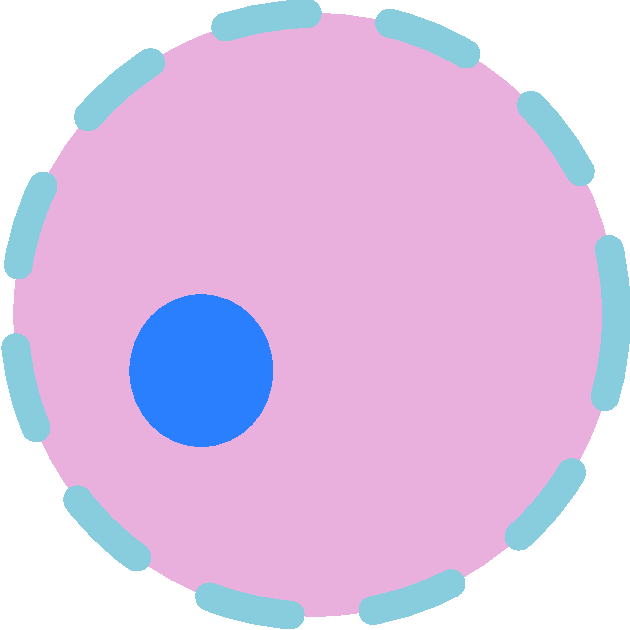
\includegraphics[scale=0.22]{images/nucleus.pdf}};
\end{code}
\end{entry}

\begin{entry}{Arc on layer}{draw layer=<layer>}{PD, AF, ER}
\begin{code}
\draw[stimulation, draw layer=background] (0,-1) -- (0,1);
\node[biological activity] {};
\end{code}
\end{entry}

Because \sbgntikz{} uses a finite number of layers, one must be careful when drawing compartments and (sub)complexes.
For example, it is by default not possible to draw a compartment inside another compartment if this latter has been drawn first.
However, it is possible to achieve that by manually adding layers:

\begin{minted}[bgcolor=gray!10]{latex}
\tikzset{sbgn/.append style={execute at begin picture={
    \pgfdeclarelayer{includedcompartments}
    \pgfsetlayers{background,compartments,includedcompartments,
        nodes,arcs,subcomplexes,subunits,attributes,main}}
    }
}
\end{minted}

Here we added a new layer \colkey{includedcompartments} just after the layer \colkey{compartments}.
Layer names should not contain any spaces.
Note that we redefined the total order as it was defined previously, just adding the new layer.
Missing one of the previously defined layer, or changing the order, could lead to compilation or drawing issues.\\

Now we can draw compartments inside other compartments, drawing the latter afterwards:

\begin{code}
\node[compartment, shape = rectangle, node layer=includedcompartments] (a) {};
\node[compartment, shape = rectangle, node layer=includedcompartments, below right = 0.5cm of a] (b) {};
\node[compartment, shape = ellipse, subunits=(a)(b)] {};
\end{code}

\section{Customizing and drawing maps effectively}
\label{sec:eff}
\subsection{Useful options for nodes and arcs}

The style of nodes and arcs (and their attributes) can be customized at will using the numerous options offered by \texttikz{}.
Following are a few options that might be useful for customizing SBGN maps.\\

\begin{entry}{Foreground color}{draw=<color>}{Nodes, Arcs}
\begin{code}
\node[generic process, draw = red] (p) {};
\node[unspecified entity, draw = blue, below = of p] (m) {};
\draw[production, draw = green] (p) -- (m);
\end{code}
\end{entry}

\begin{entry}{Background color}{fill=<color>}{Nodes}
\begin{code}
\node[unspecified entity, fill = green!120] (m) {};
\end{code}
\end{entry}

\begin{entry}{Background shading}{shade}{Nodes}
\begin{code}
\node[unspecified entity, shade, top color = green!120, bottom color = red!120] (m) {};
\end{code}
\end{entry}

\begin{entry}{Arc tip background color}{<sbgn arc>=<color>}{Arcs}
\begin{code}
\draw[modulation=red!20] (0,0) -- (2,0);
\end{code}
\end{entry}


\begin{entry}{Line width}{line width=<dimension>}{Nodes, Arcs}
\begin{code}
\node[unspecified entity, line width = 3pt] (m) {};
\draw[absolute stimulation, line width = 0.2pt] (m) -- (0cm,-3cm);
\end{code}
\end{entry}

\begin{entry}{Minimum width}{minimum width=<dimension>}{Nodes}
\begin{code}
\node[complex, minimum width = 20pt] (m) {};
\node[simple chemical, minimum width = 70pt] at (0cm,-2.5cm) (m) {};
\end{code}
\end{entry}

\begin{entry}{Minimum height}{minimum height=<dimension>}{Nodes}
\begin{code}
\node[complex, minimum height = 20pt] (m) {};
\node[simple chemical, minimum height = 70pt] at (0cm,-2cm) (m) {};
\end{code}
\end{entry}

\subsection{Positioning of nodes, arcs, and their attributes}

\texttikz{} offers two ways of positioning nodes: with absolute coordinates and relatively to other nodes.
We discourage using absolute coordinates as those cannot be changed easily through the drawing process.
Drawing maps is far easier using relative positioning.
For example, state variables can be placed using the border anchor of the entity pool node they decorate:

\begin{code}
\node[macromolecule] at (0,0) (m) {};
\node[sv] at (m.140) {val@var};
\end{code}

Here, we decided to place the state variable at an angle of 140\textdegree{} on the border of the entity pool node.
Now, if we want to change the position of the entity pool node, we don't have to change the position of the state variable:

\begin{code}
\node[macromolecule] at (0,2) (m) {};
\node[sv] at (m.140) {val@var};
\end{code}

Nodes can also be easily be placed relatively to other nodes using the \emph{positioning} \texttikz{} library, with the following syntax:

\begin{minted}[bgcolor=gray!10, breaklines]{latex}
\node[<sbgn_node>, <direction> = <distance> of <node_name>] ...;
\end{minted}

Here, \mintinline{latex}{<direction>} defines in what direction the node should be place relatively to a previously defined node named \mintinline{latex}{<node_name>}.
This direction can be unitary (\mintinline{latex}{left}, \mintinline{latex}{right}, \mintinline{latex}{above}, \mintinline{latex}{below}) or composed of two values (vertical direction first, e.g. \mintinline{latex}{above left}).
The node will be placed in that direction at the distance \mintinline{latex}{<distance>} of the border of node \mintinline{latex}{<node_name>}.
In case of a composed direction, one can define a distance for each sub-direction: \mintinline{latex}{<distance1> and <distance2>}.
If no distance is provided, the node will be placed at a distance of 1.5cm (default in \emph{sbgntikz}).
Following are some usage examples:

\begin{code}
\node[unspecified entity] (m) {};
\node[generic process, below = of m] {};
\end{code}

\begin{code}
\node[unspecified entity] (m) {};
\node[generic process, above left = 0.2cm of m] {};
\end{code}

\begin{code}
\node[unspecified entity] (m) {};
\node[generic process, below left = 2cm and 0.1cm of m] {};
\end{code}

To make the node closer to the other one, a negative distance can be defined:

\begin{code}
\node[unspecified entity] (m) {};
\node[generic process, below left = 1cm and -1cm of m] {};
\end{code}

\subsection{Bended arcs, multi-part arcs}
\index{bended arc}

\texttikz{} offers a simple way to bend arcs with the following syntax:
\begin{minted}[bgcolor=gray!10]{latex}
\draw (a) to [in=<in_angle>, out=<out_angle>] (b);
\end{minted}

where \mintinline{latex}{<in_angle>} specifies the angle at which the arc leaves the source point or node and \mintinline{latex}{<out_angle>} the angle at which the arc arrives on the target point or node.
Both angles are defined relatively to the picture's coordinate.

One can also use the following shortcut:

\begin{minted}[bgcolor=gray!10]{latex}
\draw (a) to [bend <direction>=<angle>] (b);
\end{minted}

where \mintinline{latex}{<direction>={left, right}} specifies the direction where to bend the arc and \mintinline{latex}{<angle>} the angle at which the arc leaves the source point or node.
The angle is this time defined relatively to the line passing through both points/nodes.

\begin{code}
\node[biological activity] (a) {A};
\node[biological activity, below = of a] (b) {B};
\draw[modulation] (a) to [out=-120, in=80] (b);
\draw[stimulation] (a) to [bend left=40] (b);
\draw[inhibition] (a) to [bend right=80] (b);
\end{code}

\index{multi-part arc}

It is often necessary to break arcs into muliple parts for improved readability.
\texttikz{} offers very simple operations to break arcs into horizontal and vertical sub-parts, that replace the default \mintinline{latex}{--} operation.
The \mintinline{latex}{|-} operation will produce an horizontal sub-part followed by a vertical one, and the \mintinline{latex}{-|} a vertical sub-part followed by a horizontal one.
It can also be convenient to use the \mintinline{latex}{--+} and \mintinline{latex}{--++} to draw arcs with more than two sub-parts.

\begin{code}
\node[biological activity] (a) {A};
\node[biological activity, below right = 1.5cm and 0.3 cm of a.center] (b) {B};
\draw[stimulation] (a.240) |- (b);
\draw[inhibition] (a) -| (b);
\draw[modulation] (b.240) --++ (0,-1) --++ (1,0) --++ (0,1);
\end{code}

\subsection{Nodes along paths for ER maps}

In ER maps, outcomes should be drawn along interaction or assignment arcs.
\texttikz{} provides a handy syntax to do so:

\begin{code}
\draw[interaction] (0,0) -- (3,0) node[outcome, pos = 0.7] (o) {};
\end{code}

Here, the outcome is added along the path using the \mintinline{latex}{node} command (with no \textbackslash), as if it was a normal node.
The \colkey{pos} option allows defining the distance of the node from the source of the arc relatively to the length of the arc.
Here, we placed the outcome at a distance of 70\%.
More than one outcome can be placed along an arc, by repeating the \mintinline{latex}{node} syntax:

\begin{code}
\draw[interaction] (0,0) -- (3,0) node[outcome, pos = 0.3] (o1) {} node[outcome, pos = 0.5] (o2) {} node[outcome, pos = 0.7] (o3) {};
\end{code}

One other particularity of drawing ER maps is that one might have to draw arcs targeting other arcs.
This is not straightforwardly possible in \texttikz{}, as arcs must target points or nodes.
One solution provided by \emph{sbgntikz} is to draw \colkey{anchor point} coordinates along arcs, as in the following example:

\begin{code}
\draw[interaction] (0,0) -- (3,0) coordinate[anchor point, pos = 0.5] (a);
\draw[stimulation] (1,1) -- (a);
\end{code}

Here, the \colkey{anchor point} coordinate (which is a circle with no drawing, no label and a radius of 2pt) is placed halfway along the interaction arc.\\

Often in ER maps, one wants to draw horizontal or vertical modulation arcs departing from outcomes.
These particular cases, on the other hand, can be easily achieved using \texttikz{}'s \mintinline{latex}{|-} syntax:

\begin{code}
\draw[interaction] (0,0) -- (3,0);
\draw[stimulation] (1,1) -- (1,1 |- 3,0);
\end{code}

Additional space between the tip of the modulation arc and the target arc can be added (here 2pt, that is the anchor point's default radius):

\begin{code}
\draw[interaction] (0,0) -- (3,0);
\draw[inhibition] (1,1) -- ($(1,1 |- 3,0)+(0,2pt)$);
\end{code}

Drawing vertical or horizontal modulation arcs can also be achieved using anchor points and \texttikz{}'s \mintinline{latex}{let} syntax, which allows to place the anchor point at the X-coordinate (for a vertical arc) or Y-coordinate (for an horizontal arc) of the outcome.
Following is an example:

\begin{code}
\draw[interaction] (0,0) -- (3,0) node[outcome, pos = 0.7] (o1) {};
\draw[interaction] let \p1=(o1) in (0,-2) -- (3,-2) coordinate[anchor point] (a) at (\x1,-2) node[outcome, pos = 0.3] (o2) {};
\draw[stimulation] (o1) -- (a);
\end{code}

In the second interaction, we define the point \mintinline{latex}{\p1} as being the outcome of the second interaction, and we use its X-coordinate defined as \mintinline{latex}{\x1} to place the anchor point.
More coordinates can be defined and accessed using the let command, always using the syntax \mintinline{latex}{\p}i and \mintinline{latex}{\x}i,\mintinline{latex}{\y}i:

\begin{code}
\draw[interaction] (0,0) -- (3,0) node[outcome, pos = 0.7] (o1) {};
\draw[interaction] (-0.7,-0.5) -- (1.9,-0.5) node[outcome, pos = 0.6] (o2) {};
\draw[interaction] let \p1=(o1), \p2=(o2) in (0,-2) -- (3,-2) coordinate[anchor point] (a1) at (\x1,-2) coordinate[anchor point] (a2) at (\x2,-2);
\draw[stimulation] (o1) -- (a1);
\draw[absolute inhibition] (o2) -- (a2);
\end{code}

% \section{License}
%
% \emph{sbgntikz} is free software: you can redistribute it and/or modify
% it under the terms of the GNU General Public License as published by
% the Free Software Foundation, either version 3 of the License, or
% (at your option) any later version.
%
% \emph{sbgntikz} is distributed in the hope that it will be useful,
% but WITHOUT ANY WARRANTY; without even the implied warranty of
% MERCHANTABILITY or FITNESS FOR A PARTICULAR PURPOSE.  See the
% GNU General Public License for more details.
%
% You should have received a copy of the GNU General Public License
% along with \emph{sbgntikz}.  If not, see <http://www.gnu.org/licenses/>.

\section{SBGN-ML to \texttikz{} converter}

\sbgntikz{} includes an SBGN-ML~\cite{sbgnml} to \texttikz{} converter, written in Python 3.

\subsection{Installation}
The converter depends on Matthias König's libsbgnpy library~\cite{libsbgnpy} to read SBGN-ML files.
This library can be installed using pip:

\begin{minted}[bgcolor=gray!10]{bash}
pip install libsbgnpy
\end{minted}

To install the development version, please visit libsbgnpy's \href{https://github.com/matthiaskoenig/libsbgn-python}{webpage}.

\subsection{Usage}

By default, the converter reads an input SBGN-ML file, and outputs a \texttikz{} picture.
It's usage is as follows:

\begin{minted}[bgcolor=gray!10]{bash}
./sbgnml2tikz [options] INPUT FILE
\end{minted}

If no option is supplied, the \texttikz{} picture will be output as text on the terminal's STDOUT.

Options are the following:

\begin{itemize}
    \item \mintinline[bgcolor=gray!10]{bash}{--tex=<OUTPUT FILE>}: writes the output \texttikz{} picture to a tex file
    \item \mintinline[bgcolor=gray!10]{bash}{--pdf=<OUTPUT FILE>}: renders the output \texttikz{} picture in a pdf file. This option necessitates the installation of the python package \href{https://jeltef.github.io/PyLaTeX/current/}{PyLaTeX} to compile the \texttikz{} picture.
    \item \mintinline[bgcolor=gray!10]{bash}{--no-tidy}: desactivates relative positioning. Arcs and attributes are drawn using their absolute coordinates.
    \item \mintinline[bgcolor=gray!10]{bash}{--unit=<dimension unit>}: the length unit to use. Default is ``pt'' (points). Other available units are ``cm'' (centimeters), ``in'' (inches), ``px'' (pixels).
\end{itemize}

\bibliographystyle{unsrt}
\bibliography{sbgntikz_v1_1_0}

\printindex

\end{document}
